\documentclass{standalone}
\usepackage{tikz}
%\usepackage[papersize={14cm,14cm}]{geometry}
\usetikzlibrary{chains,shapes.arrows, arrows, positioning}
\makeatletter
\tikzset{west above/.code=\tikz@lib@place@handle@{#1}{south west}{0}{1}{north west}{1}}
\tikzset{west below/.code=\tikz@lib@place@handle@{#1}{north west}{0}{-1}{south west}{1}}
\tikzset{east above/.code=\tikz@lib@place@handle@{#1}{south east}{0}{1}{north east}{1}}
\tikzset{east below/.code=\tikz@lib@place@handle@{#1}{north east}{0}{-1}{south east}{1}}
\makeatother

\begin{document}
\fontsize{8pt}{9pt}\selectfont


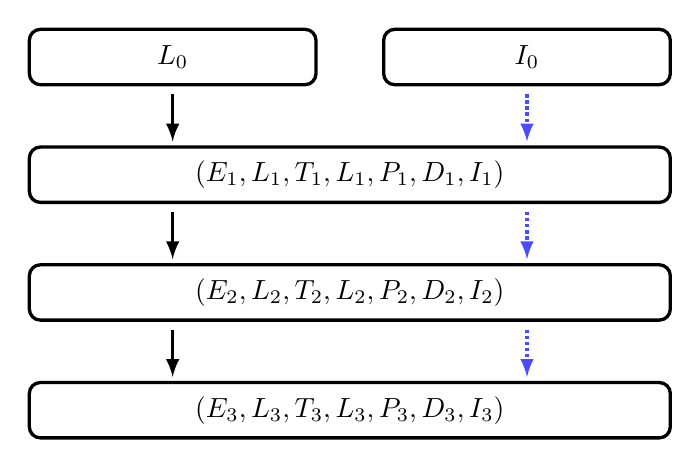
\begin{tikzpicture}[
  every node/.style={
    rectangle,
    rounded corners,
    % fill=black!10,
    draw=black, very thick,
    minimum height=2em,
    inner sep=2pt,
    text centered,
    align=center
  },
  big node/.style={text width=8cm},
  small node/.style={text width=3.5cm},
  >=latex, %Make the arrow tips latex
  myline/.style={draw, very thick,black, node distance=1.1cm},
  mylinedot/.style={draw, very thick, blue!100!black!70, densely dotted,  node distance=1cm},
  shorter/.style={shorten <=1mm,shorten >=0.5mm},
  node distance=0.75cm,
  |*/.style={to path=(\tikztostart.south) -- (\tikztostart.south|-\tikztotarget.north)},
  *|/.style={to path=(\tikztostart.south-|\tikztotarget.north) -- (\tikztotarget.north)}
  ]
\begin{scope}[every node/.append style={big node}]
  \node (B) {$(E_1,L_1,T_1,L_1,P_1,D_1,I_1)$};
  \node[below=of B] (C) {$(E_2,L_2,T_2,L_2,P_2,D_2,I_2)$};
  \node[below=of C] (D) {$(E_3,L_3,T_3,L_3,P_3,D_3,I_3)$};
\end{scope}
\begin{scope}[every node/.append style={small node}]
  \node[west above=of B] (A1) {$L_0$};
  \node[east above=of B] (A2) {$I_0$};
\end{scope}
\path[myline,shorter]  {[|*] (A1) edge[->] (B)}
                              ([shift={(-2.25cm,0)}]B.south)  edge[->] ([shift={(-2.25cm,0)}]C.north)
                              ([shift={(-2.25cm,0)}]C.south)  edge[->] ([shift={(-2.25cm,0)}]D.north)
                          %{[*|] (D)  edge[->] (E1)}
                         ;
\path[mylinedot,shorter]  {[|*] (A2) edge[->] (B) }
                             ([shift={(2.25cm,0)}]B.south)  edge[->] ([shift={(2.25cm,0)}]C.north)
                              ([shift={(2.25cm,0)}]C.south)  edge[->] ([shift={(2.25cm,0)}]D.north)
                        %  {[*|] (D) edge[->] (E2)}
                        %  (E1) edge[->] (E2)
                         ;
\end{tikzpicture}
\end{document}
